%-----------------------circuit 2--------------------------
\section{Single Phase Half Wave Uncontrolled Rectifier with RL load}

\subsection{Circuit used for simulation}

% figure that is centered on the page
\begin{figure}[h]
    \centering
    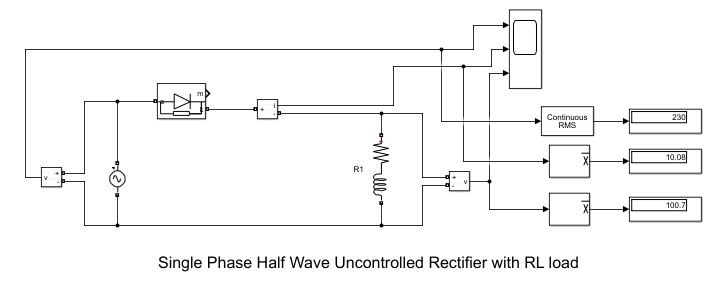
\includegraphics[width=0.7\textwidth]{images/experiment-1/circuit-diagram-simulation-02.png}
    \caption{Circuit used for simulation}
    \label{Fig_simulation_circuit_single-phase-half-wave-uncontrolled-rectifier-with-RL-load}
\end{figure}

\subsection{Components Required}

\begin{table}[h]
    \renewcommand{\arraystretch}{1.3}
    \label{table_components_required_circuit_2}
    \centering
    \begin{tabular}{|c|c|c|c|}
        \hline
        Sr. No & Parameters                     & Ratings            & Quantity \\
        \hline
        \hline
        1      & AC Single Phase Voltage Source & 230V ($ V_{rms} $) & 1        \\
        \hline
        2      & Resistor                       & 10$ \Omega $       & 1        \\
        \hline
        3      & Inductor                       & 10mH               & 1        \\
        \hline
        4      & Diode                          & -                  & 1        \\
        \hline
        5      & Voltmeter                      & -                  & 2        \\
        \hline
        6      & Ammeter                        & -                  & 1        \\
        \hline
    \end{tabular}
    \caption{Components for Single Phase Half Wave Uncontrolled Rectifier with RL load}
\end{table}


\subsection{Observations}

\begin{table}[h]
    \renewcommand{\arraystretch}{1.3}
    \label{table_observation_2}
    \centering
    \begin{tabular}{|c|c|c|}
        \hline
        Parameters                              & Theoretical Values & Simulation Values \\
        \hline
        \hline
        AC Input Voltage ($ V_{in,rms} $)       & 230V               & 230V              \\
        \hline
        Output Average Voltage ($ V_{o,avg} $)  & 103.53V            & 100.8V            \\
        \hline
        Output Average Current ($ I_{o,avg}  $) & 10.35A             & 10.08A            \\
        \hline
        AC Input Power ($ P_{AC} $)             & 2389.5 (W)         & 2318 (W)          \\
        \hline
        DC Input Power ($ P_{DC} $)             & 1071.53 (W)        & 1017 (W)          \\
        \hline
        Efficiency (\%)                         & 44.84              & 43.84             \\
        \hline
    \end{tabular}
    \caption{Observations for Single Phase Half Wave Uncontrolled Rectifier with RL load}

\end{table}


The simulated values match the theoretical values closely. However, because the load has an inductive component, the output current lags behind the output voltage. This lag causes the diode to conduct until the output current reaches zero, leading to a negative output voltage during this time. The diode stops conducting once the output current becomes zero, and the output voltage returns to zero.
The efficiency of uncontrolled rectifier with RL load is 44.84\%.
\pagebreak


\subsection{Resultant Waveforms}

% figure that is centered on the page
\begin{figure}[h]
    \centering
    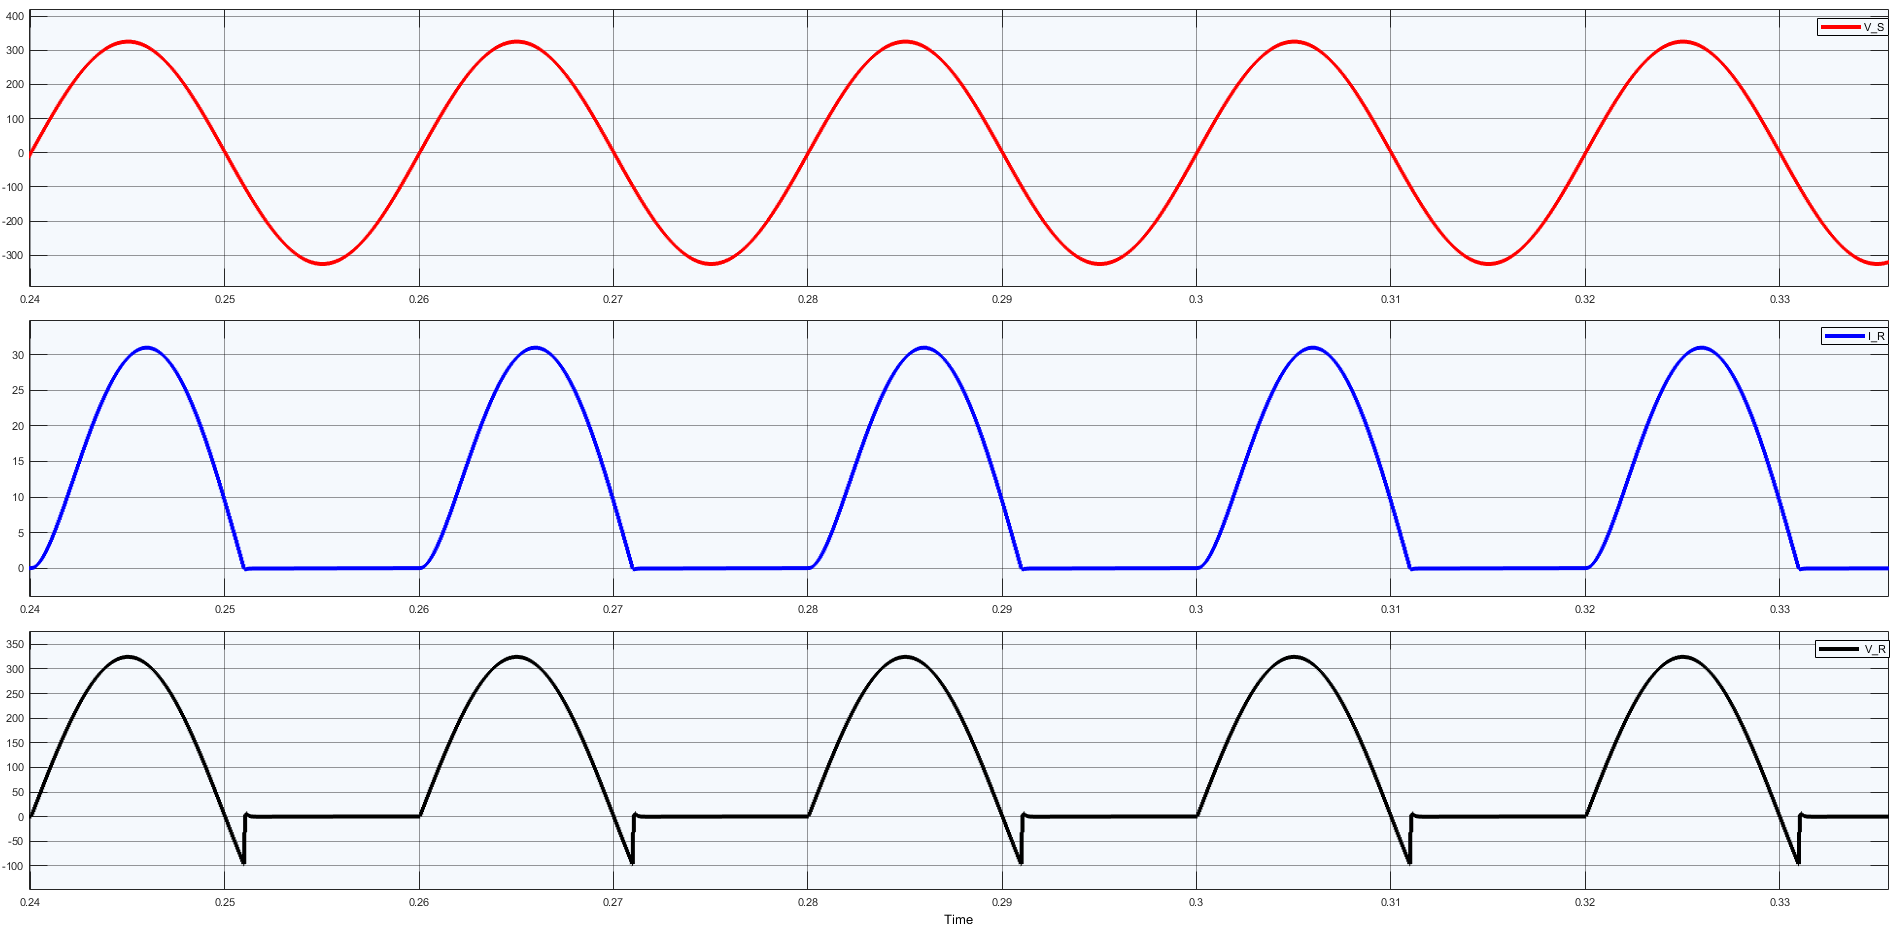
\includegraphics[width=1\textwidth]{images/experiment-1/circuit-scope-simulation-02.png}
    \caption{Scope Waveforms for Single Phase Half Wave Uncontrolled Rectifier with RL load}
    \label{Fig_waveform_single-phase-half-wave-uncontrolled-rectifier-with-RL-load}
\end{figure}

\pagebreak
